\section{Comparison With Other Deep Learning Frameworks}\label{sec:comp}

Next to TensorFlow, there exist a number of other open source deep learning
software libraries, the most popular being Theano, Torch and Caffe. In this
section, we explore the \emph{qualitative} as well as \emph{quantitative}
differences between TensorFlow and each of these alternatives. We begin with a
``high level'' qualitative comparison and examine where TensorFlow diverges or
overlaps conceptually or architecturally. Then, we review a few sources of
quantitative comparisons and state as well as discuss their results.

\subsection{Qualitative Comparison}\label{sec:comp-quality}

The following three paragraphs compare Theano, Torch and Caffe to TensorFlow,
respectively. Table \ref{tab:comp} provides an overview of the most important
talking points.

\subsubsection{Theano}\label{sec:comp-quality-theano}

Of the three candidate alternatives we discuss, Theano, which has a Python
frontend, is most similar to TensorFlow. Like TensorFlow, Theano's programming
model is \emph{declarative} rather than \emph{imperative} and based on
computational graphs. Also, Theano employs symbolic differentiation, as does
TensorFlow. However, Theano is known to have very long graph compile times as it
translates Python code to C++/CUDA \cite{theano}. In part, this is due to the
fact that Theano applies a number of more advanced graph optimization algorithms
\cite{theano}, while TensorFlow currently only performs common subgraph
elimination. Moreover, Theano's visualization tools are very poor in comparison
to TensorBoard. Next to built-in functionality to output plain text
representations of the graph or static images, a plugin can be used to generate
slightly interactive HTML visualizations. However, it is nowhere near as
powerful as TensorBoard. Lastly, there is also no (out-of-the-box) support for
distributing the execution of a computational graph, while this is a key feature
of TensorFlow.

\subsubsection{Torch}\label{sec:comp-quality-torch}

One of the principle differences between Torch and TensorFlow is the fact that
Torch, while it has a C/CUDA backend, uses Lua as its main frontend. While
Lua(JIT) is one of the fastest scripting languages and allows for rapid
prototyping and quick execution, it is not yet very mainstream. This implies
that while it may be easy to train and develop models with Torch, Lua's limited
API and library ecosystem can make industrial deployment harder compared to a
Python-based library such as TensorFlow (or Theano). Besides the language
aspect, Torch's programming model is fundamentally quite different from
TensorFlow. Models are expressed in an imperative programming style and not as
declarative computational graphs. This means that the programmer must, in fact,
be concerned with the order of execution of operations. It also implies that
Torch does not use symbol-to-symbol, but rather symbol-to-number differentiation
requiring explicit forward and backward passes to compute gradients.

\subsubsection{Caffe}\label{sec:comp-quality-caffe}

Caffe is most dissimilar to TensorFlow --- in various ways. While there exist
high-level MATLAB and Python frontends to Caffe for model creation, its main
interface is really the Google Protobuf ``language'' (it is more a fancy, typed
version of JSON), which gives a very different experience compared to
Python. Also, the basic building blocks in Caffe are not operations, but entire
neural network layers. In that sense, TensorFlow can be considered fairly
low-level in comparison. Like Torch, Caffe has no notion of a computational
graphs or symbols and thus computes derivatives via the symbol-to-number
approach. Caffe is especially well suited for development of convolutional
neural networks and image recognition tasks, however it falls short in many
other state-of-the-art categories supported well by TensorFlow. For example,
Caffe, by design, does not support cyclic architectures, which form the basis of
RNN, LSTM and other models. Caffe has no support for distributed
execution\footnote{\url{https://github.com/BVLC/caffe/issues/876}}.

\begin{table}[h!]
  \begin{tabular}{llllc}
    \textbf{Library} & \textbf{Frontends} &
    \textbf{Style} &
    \textbf{Gradients} &
    \specialcell{\textbf{Distributed}\\\textbf{Execution}}
    \\ \toprule
    TensorFlow & Python, C++\textsuperscript{\dag} &
    Declarative & Symbolic & $\checkmark$\textsuperscript{\ddag}
    \\
    Theano & Python & Declarative & Symbolic & $\times$
    \\
    Torch & LuaJIT & Imperative & Explicit & $\times$
    \\
    Caffe & Protobuf & Imperative & Explicit & $\times$
    \\ \bottomrule
  \end{tabular}
  \begin{tabular}{l}
    \textsuperscript{\dag} Very limited API.
    \\
    \textsuperscript{\ddag} Starting with TensorFlow 0.8, released in April 2016
    \cite{tensorflowdist}.
  \end{tabular}
  \caption{A table comparing TensorFlow to Theano, Torch and Caffe in several
    categories.}
  \label{tab:comp}
\end{table}

\subsection{Quantitative Comparison}\label{sec:comp-quantity}

We will now review three sources of quantitative comparisons between TensorFlow
and other deep learning libraries, providing a summary of the most important
results of each work. Furthermore, we will briefly discuss the overall trend of
these benchmarks.

The first work, \cite{bosch}, authored by the Bosch Research and Technology
Center in late March 2016, compares the performance of TensorFlow, Torch, Theano
and Caffe (among others) with respect to various neural network architectures.
Their setup involves Ubuntu 14.04 running on an Intel Xeon E5-1650 v2 CPU @ 3.50
GHz and an NVIDIA GeForce GTX Titan X/PCIe/SSE2 GPU. One benchmark we find
noteworthy tests the relative performance of each library on a slightly modified
reproduction of the LeNet CNN model \cite{lenet}. More specifically, the authors
measure the forward-propagation time, which they deem relevant for model
deployment, and the back-propagation time, important for model training. We have
reproduced an excerpt of their results in Table \ref{tab:bosch}, where we show
their outcomes on (a) a CPU running 12 threads and (b) a GPU. Interestingly, for
(a), TensorFlow ranks second behind Torch in both the forward and backward
measure while in (b) TensorFlow's performance drops significantly, placing it
\emph{last} in both categories. The authors of \cite{bosch} note that one reason
for this may be that they used the NVIDIA cuDNN \emph{v2} library for their GPU
implementation with TensorFlow while using cuDNN \emph{v3} for the others. They
state that as of their writing, this was the recommended configuration for
TensorFlow\footnote{As of TensorFlow 0.8, released in April 2016 and thus after
  the publication of \cite{bosch}, TensorFlow now supports cuDNN v4, which
  promises better performance on GPUs than cuDNN v3 and especially cuDNN v2.}.

\begin{table}
  \begin{subfigure}[h]{0.49\textwidth}
    \centering
    \begin{tabular}{ccc}
      \textbf{Library} & \textbf{Forward (ms)} & \textbf{Backward (ms)}
      \\ \toprule
      TensorFlow & 16.4 & 50.1
      \\
      Torch & \textbf{4.6} & \textbf{16.5}
      \\
      Caffe & 33.7 & 66.4
      \\
      Theano & 78.7 & 204.3
      \\ \bottomrule
    \end{tabular}
    \caption{CPU (12 threads)}
  \label{tab:bosch-a}
  \end{subfigure}

  \vspace{0.5cm}

  \begin{subfigure}[h]{0.49\textwidth}
    \centering
    \begin{tabular}{ccc}
      \textbf{Library} & \textbf{Forward (ms)} & \textbf{Backward (ms)}
      \\ \toprule
      TensorFlow & 4.5 & 14.6
      \\
      Torch & \textbf{0.5} & 1.7
      \\
      Caffe & 0.8 & 1.9
      \\
      Theano & \textbf{0.5} & \textbf{1.4}
      \\ \bottomrule
    \end{tabular}
    \caption{GPU}
    \label{tab:bosch-b}
  \end{subfigure}
  \caption{This table shows the benchmarks performed by \cite{bosch}, where
    TensorFlow, Torch, Caffe and Theano are compared on a LeNet model
    reproduction \cite{lenet}. \ref{tab:bosch-a} shows the results performed
    with 12 threads each on a CPU, while \ref{tab:bosch-b} gives the outcomes on
    a graphics chips.}
  \label{tab:bosch}
\end{table}

The second source in our collection is the \emph{convnet-benchmarks} repository
on GitHub by Soumith Chintala \cite{convnet-bench}, an artificial intelligence
research engineer at Facebook. The commit we reference\footnote{Commit sha1
  hash: 84b5bb1785106e89691bc0625674b566a6c02147} is dated April 25,
2016. Chintala provides an extensive set of benchmarks for a variety of
convolutional network models and includes many libraries, including TensorFlow,
Torch and Caffe in his measurements. Theano is not present in all tests, so we
will not review its performance in this benchmark suite. The author's hardware
configuration is a 6-core Intel Core i7-5930K CPU @ 3.50GHz and an NVIDIA Titan
X graphics chip running on Ubuntu 14.04. Inter alia, Chintala gives the forward
and backward-propagation time of TensorFlow, Torch and Caffe for the AlexNet CNN
model \cite{alexnet}. In these benchmarks, TensorFlow performs second-best in
both measures behind Torch, with Caffe lagging relatively far behind. We
reproduce the relevant results in Table \ref{tab:convnet}.

\begin{table}
  \centering
  \begin{tabular}{ccc}
    \textbf{Library} & \textbf{Forward (ms)} & \textbf{Backward (ms)}
    \\ \toprule
    TensorFlow & 26  & 55
    \\
    Torch & \textbf{25} & \textbf{46}
    \\
    Caffe & 121 & 203
    \\
    Theano & \textendash & \textendash
    \\ \bottomrule
  \end{tabular}
  \caption{The result of Soumith Chintala's benchmarks for TensorFlow, Torch and
    Caffe (not Theano) on an AlexNet ConvNet model \cite{alexnet,
      convnet-bench}.}
  \label{tab:convnet}
\end{table}

Lastly, we review the results of \cite{theano}, published by the Theano
development team on May 9, 2016. Next to a set of benchmarks for four popular
CNN models, including the aforementioned AlexNet architecture, the work also
includes results for an LSTM network operating on the Penn Treebank dataset
\cite{penntreebank}. Their benchmarks measure words processed per second for a
small model consisting of a single 200-unit hidden layer with sequence length
20, and a large model with two 650-unit hidden layers and a sequence length of
50. In \cite{theano} also a medium-sized model is tested, which we ignore for
our review. The authors state a hardware configuration consisting of an NVIDIA
Digits DevBox with 4 Titan X GPUs and an Intel Core i7-5930K CPU. Moreover, they
used cuDNN v4 for all libraries included in their benchmarks, which are
TensorFlow, Torch and Theano. Results for Caffe are not given. In their
benchmarks, TensorFlow performs best among all three for the small model,
followed by Theano and then Torch. For the large model, TensorFlow is placed
second behind Theano, while Torch remains in last place. Table
\ref{fig:theano-results} shows these results, taken from \cite{theano}.

\begin{figure}
  \centering
  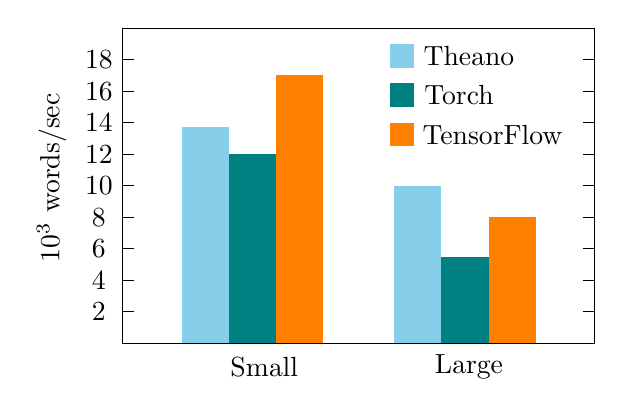
\begin{tikzpicture}
    % Frame
    \draw (0, 0) rectangle (6, 4);

    % Ticks + Scale
    \foreach \i in {2, 4, ..., 18} {
      % Left
      \draw (0, {\i / 5}) -- ++(+0.15, 0);
      % Right
      \draw (5.85, {\i / 5}) -- ++(+0.15, 0);
      % Labels
      \draw (-0.3, {\i / 5}) node {\i};
    }

    % Legend
    \draw (-0.9, 2.1) node [rotate=90] {$10^3$ words/sec};

    \fill [SkyBlue] (3.4, 3.5) rectangle ++(0.3, 0.3);
    \draw (4.4, 3.65) node {Theano};

    \fill [teal] (3.4, 3) rectangle ++(0.3, 0.3);
    \draw (4.275, 3.15) node {Torch};

    \fill [orange] (3.4, 2.5) rectangle ++(0.3, 0.3);
    \draw (4.7, 2.65) node {TensorFlow};


    %%% Small Model %%%

    % Theano
    \fill [SkyBlue] (0.75, 0) rectangle ++(0.6, 2.75);
    % Torch
    \fill [teal] (1.35, 0) rectangle ++(0.6, 2.4);
    % TensorFlow
    \fill [orange] (1.95, 0) rectangle ++(0.6, 3.4);

    % Label
    \draw (1.8, -0.3) node {Small};

    %%% Large Model %%%

    % Theano
    \fill [SkyBlue] (3.45, 0) rectangle ++(0.6, 2);
    % Torch
    \fill [teal] (4.05, 0) rectangle ++(0.6, 1.1);
    % TensorFlow
    \fill [orange] (4.65, 0) rectangle ++(0.6, 1.6);

    % Label
    \draw (4.4, -0.3) node {Large};

  \end{tikzpicture}
  \caption{The results of \cite{theano}, showing a comparison of TensorFlow,
    Theano and Torch on an LSTM model for the Penn Treebank dataset
    \cite{penntreebank}. On the left the authors tested a small model with a
    single hidden layer of 200 units; on the right they use two layers with 650
    units each. }
  \label{fig:theano-results}
\end{figure}

When TensorFlow was first released, it performed poor on benchmarks, causing
disappointment within the deep learning community. Since then, new releases of
TensorFlow have emerged, bringing with them improving results. This is reflected
in our selection of works. The earliest of the three sources, \cite{bosch},
published in late March 2016, ranks TensorFlow consistently uncompetitive
compared to Theano, Torch and Caffe. Released almost two months later,
\cite{convnet-bench} ranks TensorFlow comparatively better. The latest work
reviewed, \cite{theano}, then places TensorFlow in first or second place for
LSTMs and also other architectures discussed by the authors. We state that one
reason for this upward trend is that \cite{theano} uses TensorFlow with cuDNN v4
for its GPU experiments, whereas \cite{bosch} still used cuDNN v2. While we
predict that TensorFlow will improve its performance on measurements similar to
the ones discussed in the future, we believe that these benchmarks --- also
today --- do not make full use of TensorFlow's potential. The reason for this is
that all tests were performed on a \emph{single} machine. As we reviewed in
depth in section \ref{sec:model-exec}, TensorFlow was built with massively
parallel distributed computing in mind. This ability is currently unique to
TensorFlow among the popular deep learning libraries and we estimate that it
would be advantageous to its performance, particularly for large-scale
models. We thus hope to see more benchmarks in literature in the future, making
better use of TensorFlow's many-machine, many-device capabilities.

%%% Local Variables:
%%% mode: latex
%%% TeX-master: "../paper"
%%% End: